\chapter{When time is the essence}

When time is the essence for optimal behavior, animals must make use of some inner representation to behave. Because time is an implicit variable in perception, computations are needed to abstract time from series of static perceptions, movements, memories, or anything else that may serve this purpose. A common set of computations and respective mechanisms are used by the nervous system to guide temporal behavior, and seems to be consistent between humans and mice. The recruited mechanisms are dependent on the size of the time interval under consideration, and possibly on other characteristics of the task. To unravel these mechanisms, many tasks have been developed by the timing community.

To make sense of results in a wide range of tasks, there are various cognitive models for timing learning and performance, but although they make assumptions about learning, they are commonly assessed only via proficient behavior, due to difficulties in recording animals through the learning process. Our group developed a variant of DRRD task, in which animals learn in the course of a single session, and we record neural activity in two regions associated with timing in the recent literature: the medial Pre Frontal Cortex (mPFC) and the Striatum (STR). We aim to shed some light into the process of learning to time by studying how time representations develop in these areas.

We found that, from the onset of training, there is activity at the mPFC consistent with time representation. This representation weakens in trained animals, a result consistent across two groups of animals from distinct laboratories. In the opposite direction, STR has no detectable representation of time at the beginning of training, but features this representation after training. This results can be seen in figure \ref{fig:time_representation_str_pfc}, where decoding performance is used as a surrogate for time representation.

We found that, from the onset of training, there is activity at the mPFC consistent with time representation. This representation weakens in trained animals, a result consistent across two groups of animals from distinct laboratories. In the opposite direction, STR has no detectable representation of time at the beginning of training, but features this representation after training. This results can be seen in figure \ref{fig:time_representation_str_pfc}, where decoding performance is used as a surrogate for time representation.

\begin{figure}
    \centering
    \begin{tabular}{cc}

    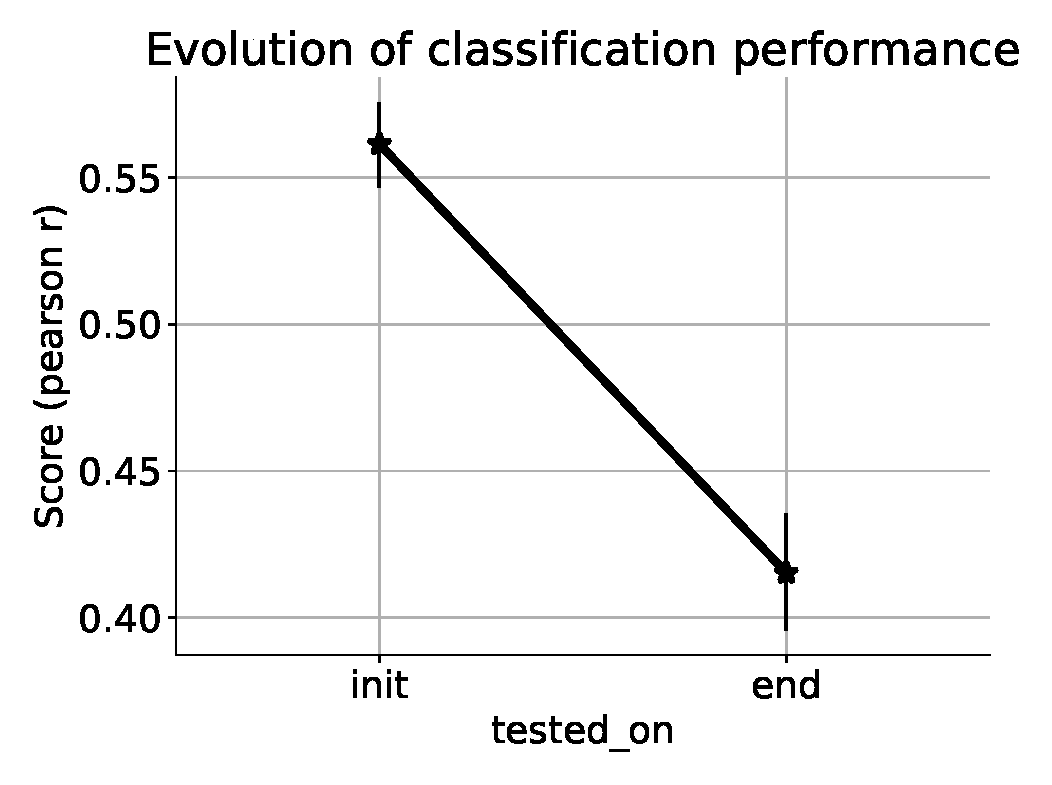
\includegraphics[width=7cm]{figures/PFC_init_vs_end.eps}
    & 
    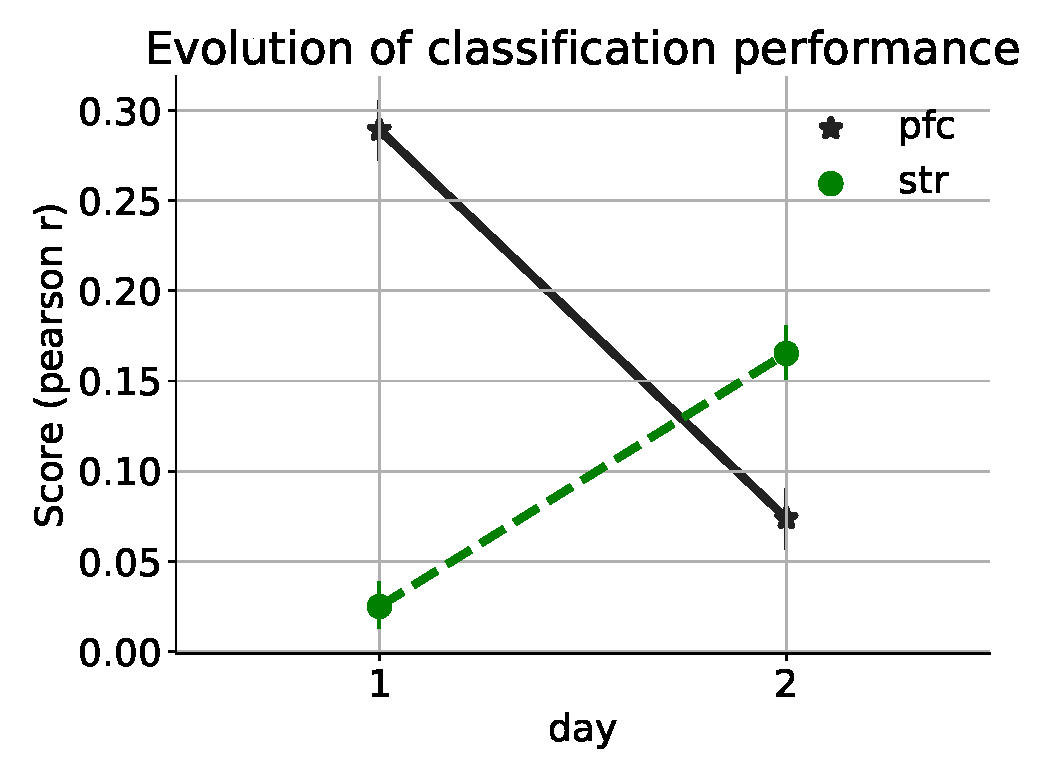
\includegraphics[width=7cm]{figures/STR_PFC_day1_vs_day2_evo.eps}
    \end{tabular}
    
    \caption[Striatum representation enhancement follows PFC's deterioration]{Striatum representation enhancement follows PFC's deterioration. Left: Group 1 at first vs second half of session. Right: Group 2, in different days.}
    \label{fig:time_representation_str_pfc}
\end{figure}

We discuss how this results relate to the already established Dual Process framework for learning.


This work has three kinds of contribution: 
\begin{enumerate}
    \item Methodology: We provide rationale for method choices, grounded on comparisons made available in the corresponding chapters. 
    
    \item Results: Analysis applied to data from our research group, giving results such as the central one aforementioned, are thorougly discussed.
    
    \item Theory: Contemporary discussions from relevant areas are brought in, and the work contextualized in multiple levels.
\end{enumerate}


% 1 paragraph discussion
% 1 small paragraph conclusion
